\section{Study Design and Data Collection}

  As a computer expert with social skills needing to design and develop an app for an unfamiliar cultural and socio-economic context, it was needed to quickly become a good designer. The technical aspect of the project was but one. It was needed to learn how to develop hybrid apps in JavaScript that worked offline, and had an online back-end. However, those are merely the technical demands.

  It was needed to quickly become a good designer, not mainly from a perspective of graphic design or interaction design, but \textit{how} to explore, design, and implement what the user needs from the requirements "fun, user-friendly, and good for learning". There was also a need to evaluate the effectiveness of the implementations, to assess learning and the interaction design aspects of desirability, utility, usability and pleasurability. The approach used to learn design from these perspectives was to read extensive literature, consult a diverse set of experts, and be humble and curious in interactions with the end-users and stakeholders. In the following section, the creation and implementation for a suitable design process is described, together with the study design and data collection for each iteration of the project.

%Har gått igenom planeringsrapporten lite noggrannare idag och ser två saker som vi kanske ska borde fånga upp under arbetets gång.

% Under 2 Purpose står det ett upplevelsemål från Young Drive. Bör vi mäta detta upplevelsemål om det stämmer med deltagarnas faktiska upplevelse, d v s ska vi försöka få in det under 3 Research Questions?

% På våra avstämningsmöten borde vi också följa upp dina Research Questions så att kundinteraktionerna och servicedesignmetoden tyligt leder dig framåt mot dessa mål.
%* Reflektioner på vilka designprinciper som bör väljas? (utifrån kundinteraktioner)
%* Reflektioner angående tekniska begränsningar?
%* Reflektioner på processen?

\subsubsection{Creation of Design Process}
As there was a unfamiliar target group - mostly young Ugandians with little or no experience of smartphones - service design thinking would benefit true understanding of cultural context and in-depth empathy for the end users.

Tools and methodology in service design were chosen with the help of Expedition Mondial in Stockholm, who provided education and coaching.

At the same time, the end result would be a digital artefact (an app), which is not common in service design.

While this product could be though of as a service, the tools and methodology would benefit to borrow from Agile methodology and Interaction design.

I'm the computer expert kind of designer \cite{lowgren}, adjusted to agile methodology and interaction design, but aspiring to be a socio-technical expert. Expedition Mondial are experienced with service design, aspiring to be more of computer experts.

This led to the joined development of a Digital Service Design method, co-created by the both.

%Expedition Mondial helped with a method for creating a MVP of the digital support for the coaches, so that the app was developed from the perspective of the end users and the education and a "learning by doing" mentality.

%The suggested design process was designed with them after a start-up meeting on Skype, and an education day in Stockholm. During that day a crash course in service design was given, then creating a common plan for the future work based on my needs (see Appendix: Original Time Plan \todo{Add reference}). They also recommended service design literature. These were the methods chosen in each iteration.

The result is that the design and development phase in Uganda is an iterative process with the human in focus. The process is built on top of service design process and methodology, while in-line with digital design practices.

\subsubsection{Implementation of Design Process}
There were four iterations. The first iteration follows Service Design, not starting the app development, while the other three follows the new methodology, Digital Service Design.

In iteration 1, there is a very broad scope, without digital focus, where iteration 2, 3 and 4 introduces and narrows down the project into a digital solution.

Expedition Mondial gave support in each iteration, helping with refinements of each iteration as learnings happened along the way, and they were able to educate me during the different stages with methodologies whenever necessary.


%\subsection{Implementation of Methods for Data Collection and Data Analysis}

This section describes the implementation of methods for each iteration's interactions, in regards to collecting and analysing qualitative and quantitative data. Figure \ref{fig:methods} is made to assist the reader in the iterations' different focuses.

%study design, application development, and for data analysis theory.

\begin{figure}[h]
    \centering
    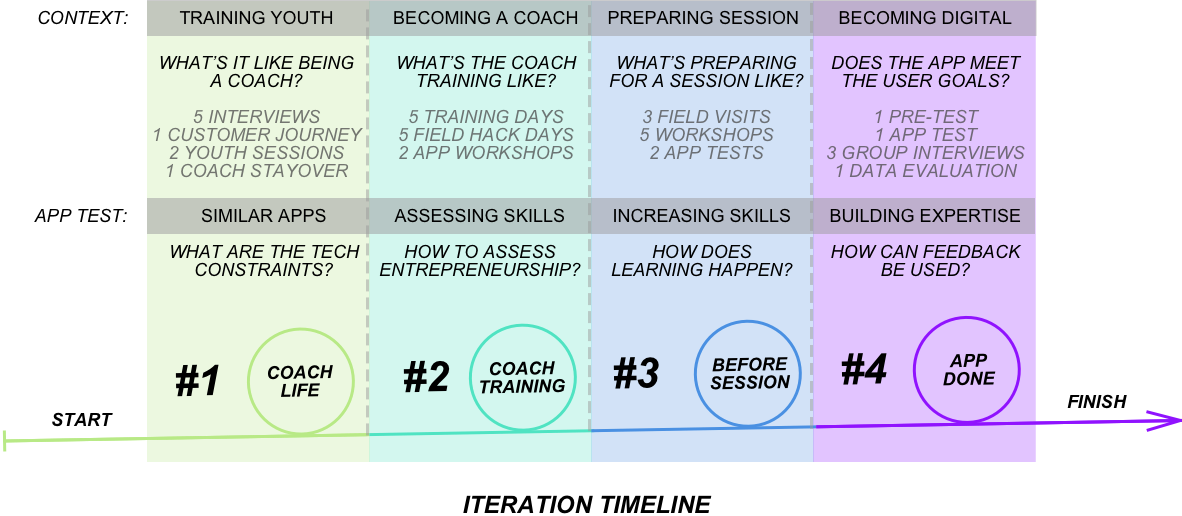
\includegraphics[width=1.0\textwidth]{iterativeprocess2.png}
    \caption{Each of the four iterations had a unique context, app test focus, and research focus. The loops is meant to remind that an iteration consists of three steps before Interactions with the coaches: Insights, Ideation and Trigger material. For more information, see section \ref{digital-service-design} Digital Service Design.}
    \label{fig:methods}
\end{figure}

%Methods w/ Analysis
%----
%
%5 Interviews - Notes - Questionnaire for Customer Journey
%1 Customer Journey - Clustering - Personas
%2 Youth Sessions - Shadowing - Needs
%1 Coach Stayover - Empathy - Design Ethnography
%
%5 Training Days - Observations - Understanding entrepreneurship training
%5 Hackathon Days - Interviews - Notes and Sketches
%2 App Workshops - Co-Creation/Co-Refinement - Sketches and Needs
%
%3 Field
%
%Acitivity
%App test observations (group)
%
%App test observation (individual)
%- Affective reactions (5 Why's, think aloud)
%
%Analysis: Interaction design evaluation (desirability, usability, utility, %pleasurability)
%
%Customer Journey Map
%- Activities
%- Behaviour
%
%Written responses (individual)
%- Right/wrong
%- Time
%- Number of tries
%
%Interviews
%- New insights
%
%Data Collection w/ Analysis
%----
%
%Customer Journey Map w/ clustering
%
%Pre-study w/ Quantative analysis
%
%Written quiz responses w/ Quantative analysis
%
%Digital quiz responses / Quantative analysis + Statistical analysis + %Parallell coordinates
%
%Quiz questions 1 w/ Bloom analysis
%Quiz questions 2 w/ Bloom analysis

%\input{implementation/iteration-1}

%\input{implementation/iteration-2}

%\input{implementation/iteration-3}

%\input{implementation/iteration-4}


\subsection{Iteration 1: Uganda Coach Visit}

% How was this iteration designed?

Following the service design sequencing, the first iteration had a very broad scope and truly is a service design iteration: "From your perspective, what is it like being a coach?". \footnote{A coach meaning either a Community Based Trainer (carrying out all the trainings), or a YoungDrive coach, depending on who was asked the question.} \cite{lowgren} was used how to start the project, meaning that the purpose was to get a preliminary understanding of all important aspects, and build relationships with all stakeholders.

%The project started with a startup meeting with Shifteh from Plan International in Kampala, together with Iliana. From there, I did research and met with Grameen Foundation and Designers Without Borders, before going to Tororo to research "What's it like being a YoungDrive coach?", and determining how advanced an app could be to solve challenges that the coaches face.

Insights depended heavily on interviews with all the stakeholders  (2 with Plan International, 3 with YoungDrive), and local experts (1 visit each at Grameen Foundation and Designers without Borders, 1 workshop with Mango Tree), since no Interactions with users had been made yet. Also, knowledge and connections were made with the Kampala tech scene as much as possible, from the new home and office in Kampala, working at the tech hub and co-working space Hive Colab.

Ideation were about creating a questionnaire guide for the interviews, a co-creation workshop using "Customer Journey Map", and identifying how the app test should be designed to test their existing knowledge (and be informed of the design preferences of the YoungDrive app).

Trigger material was the finished questionnaire guide (constructed with Expedition Mondial) a written plan for the co-creation workshop ("A day as a coach"), and a written plan for testing the quiz app Quizoid and the language learning app Duolingo, and a schedule for the interactions.

The interactions were focused on design ethnology, getting to know and learn from people in a different culture, namely the coaches. The focus was on the their needs, motivations, and context.

To accomplish these, four days were spent in Tororo, with one day of travel. There were four face-to-face-interviews,
one meeting with Plan, one meeting with the local partners, two workshops, one coach stay-over, and two youth session visits (one of the youth sessions are observable via figure \ref{fig:youthsession}.

\begin{figure}[h]
    \centering
    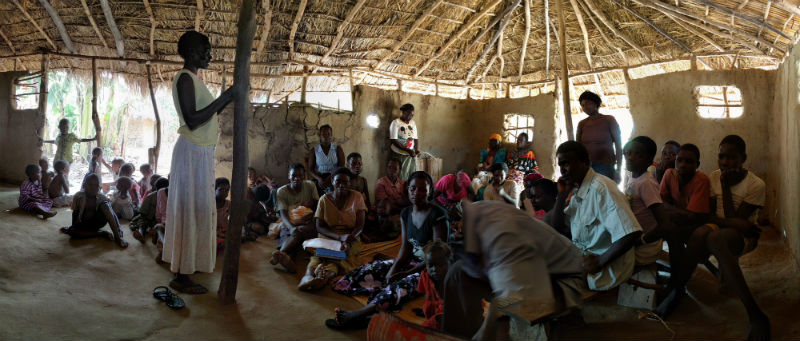
\includegraphics[width=0.7\textwidth]{youthsessionSmall.jpg}
    \caption{Photo from the location where one of the youth sessions were held. Here, a CBT in Tororo teaches youth in basic sales and marketing.}
    \label{fig:youthsession}
\end{figure}


\subsection{Iteration 2}

This time, the iteration has a more detailed scope, with a hypothesis on what needs the app should meet in the end, and create lo-fi and hi-fi trigger material to meet those needs.

A co-creation workshop started the interactions, followed by repeated app tests at minimum one session per day, always followed by a feedback round, so the app and the tomorrow's question set creation could be improved for the next day. At the end of the week, there was a co-refinement workshop of the current hi-fi material, and also lo-fi material for the new version of the app.

\subsubsection*{Creation of questions}
Project leader Josefina in Zambia refined Iliana's first question sets, prepared for my visit in Zambia. Josefina created question sets with Bloom at the back of her head, also taking into account the structure and the order of the coach manuals, what it means being a coach within the topic, and lastly scenarios.

\subsubsection{Trigger material used}
A hi-fi trigger material was done, a very basic quiz app, keeping it as simple as possible (see Application Implementation, Iteration 2). All of the devices (tablets and smartphones) that I had available were brought to Zambia.

I added Josefina's questions to the app, and installed the app to all of the devices. This process was repeated for all the days, Sunday-Friday.

\subsubsection{Design workshop \#1 in Zambia}
The coach training started with me having a design workshop with the coaches, not showing them the app that I had created. The co-creation workshop was made to identify important functionality in the minds of the coaches.

\begin{enumerate}
\item Since the knowledge about smartphones and apps were low, I started by introducing these topics.
\item All were familiar with Facebook, so thus I showed the Facebook app. Me wanting to know what the app would look like if the coaches would have designed the app, I first needed to train them how to design an app via drawing wireframes.
\item Using postits, they started with during limited time drawing the start view from the Facebook app.
\item Then, they were asked to draw what they thought happened on the friend icon click, drawing the view on another postit.
\item Then, the mission of the YoungDrive app was described. They were then divided into two teams, having limited time to draw the best imaginable YoungDrive coach quiz app they could. First, they designed the app from the top of their heads. They then pitched their results to each other.
\item On the next iteration, they were to suggest and design improvements how the app should be designed to improve learning, not only assessment. They then again pitched their results to each other.
\end{enumerate}

\subsubsection{Assessment via quiz}
At the end of each day, the app was used to test the coaches' knowledge. Each coach got either a smartphone, tablet or computer. The coach first took the quiz for the most recent session, and could then choose what to do next.

As there were no back-end developed, Josefina by hand documented the scores of each coach, writing the name of the coach, the session, number of correct answers, and what questions had been answered wrong.

Josefina then, when planning the next day, looked at the statistics, looking for trends that would inform the sessions for the following day.

She also evaluated the quality of the questions, before creating the new question sets for the next day.

\subsubsection{Experimenting with quiz before or after the session}
Since the coaches appreciated the app so much, we felt tempted to try what would happen with fun and learning if we tried using the app \textit{before} a session instead of only after. During the rest of the week, we continued, finally finding preferences and tendencies from the coaches, via observation, interviews, and survey.

\subsubsection{Experimenting with design of questions}
During the week, extra tests were done to test the following:

\begin{itemize}
\item Number of questions per quiz
\item Single-answer questions or multiple-answer questions
\item Framing of questions
\item Challenge level of questions
\item Determining what made a question hard
\end{itemize}

\subsubsection{Interviews with Josefina}
At the end of each day, an evaluation interview was held with Josefina. At the end of the week, a final interview was held.

At the end of Day 5, Josefina and I discussed what it would look like to not record the answers manually, but pushing the results online. A co-creation workshop was held, where she drew an Educator Dashboard.


\subsection{Iteration 3}

Because of the many research and functionality needs, the study design of Iteration 3 became very important. A lot of development and ideation needed to be done.

\subsubsection{Iteration 3: Purpose}
Iteration 3 had an even more detailed scope. Since the app now succeeds with the first use case, the coach training, now the focus could be on "learning at distance".

\subsubsection{Pedagogical model}
It was chosen that "Are you sure?" + Improve would be included in the hi-fi material, a flip-card approach would be tested as a lo-fi material, and to "record answer via voice" could only be presented as an idea during a field interview (experts said there would be usability issues, and the 1st-time smartphone user agreed). The Gold/Silver/Bronze method was included into the hi-fi material.

\subsubsection{Test on a Kampala entrepreneurship student}
Also, instead of only testing the app in Tororo, a test was held in Kampala, to get feedback from an entrepreneurship student.

\subsubsection{Test in Tororo}
As Plan International staff are not allowed to support visiting coaches in the field during local elections, the co-project leaders in Tororo were consulted to carry out the field trips, so that it was still possible to attend the youth group meetings.

For the interactions, a big app test was held, a group interview was held, and then they were divided into co-creation workshop groups, with a presentation in the end.

%Before the workshop, the wished functionality and goals were well formulated. It was also discussed beforehand how to best design the workshop, together with Linköping University and Expedition Mondial.

There was another partner meeting, with Plan International and Community Vision present. There was an app test with all of the coaches, "Testing the YoungDrive coach app", followed up by splitting into six workshop groups based on solving different problems discovered during the test.

The following day, there were three field visits to CBTs, observing how they prepared themselves for a youth session, and then testing the app for assessing and becoming prepared for a session.

After the app tests, it was tested with a lo-fi prototype that the coach thinks aloud about the question, \textit{before} receiving the multiple-choice answers. This approach proved to be great for learning, and could be a great addition to the hi-fi material. Interestingly, this test was done as a live quiz, and if the interviewee could not answer the question directly, the audience were asked and tested if they knew the answer (raised hands), and if nobody knew the answer, it was tested which of the multiple-choice alternatives they found most likely.

During the afternoon, we divided into 5 groups focusing on improving the app experience for the coaches.

On Wednesday, the coaches from the field visits were gathered for a workshop. The purpose was to see how they acted when given the challenge: "Get 100\% correct answers in one go, on the hardest quiz". A co-creation workshop ("Educator Dashboard") was held in parallel, with 3 CBTs and 1 project leader respectively.


\subsection{Iteration 4: Uganda Summative Test}

The focus of iteration 4 was a summative test. First, a pre-test was carried out in paper, including questions about the coach and an entrepreneurship quiz, based on a well-known study \citep{general-entrepreneurship-quiz}, see Appendix \ref{cha:pre-test}. During the test, this was the first time that the app could send data to the server. Data was sent whenever a quiz was started, and whenever a quiz was finished. The group was divided into two, the ones who brought manuals and they who did not. Those that had brought manuals, could use these with the app, see figure \ref{fig:appevaluation}.

\begin{figure}[h]
    \centering
    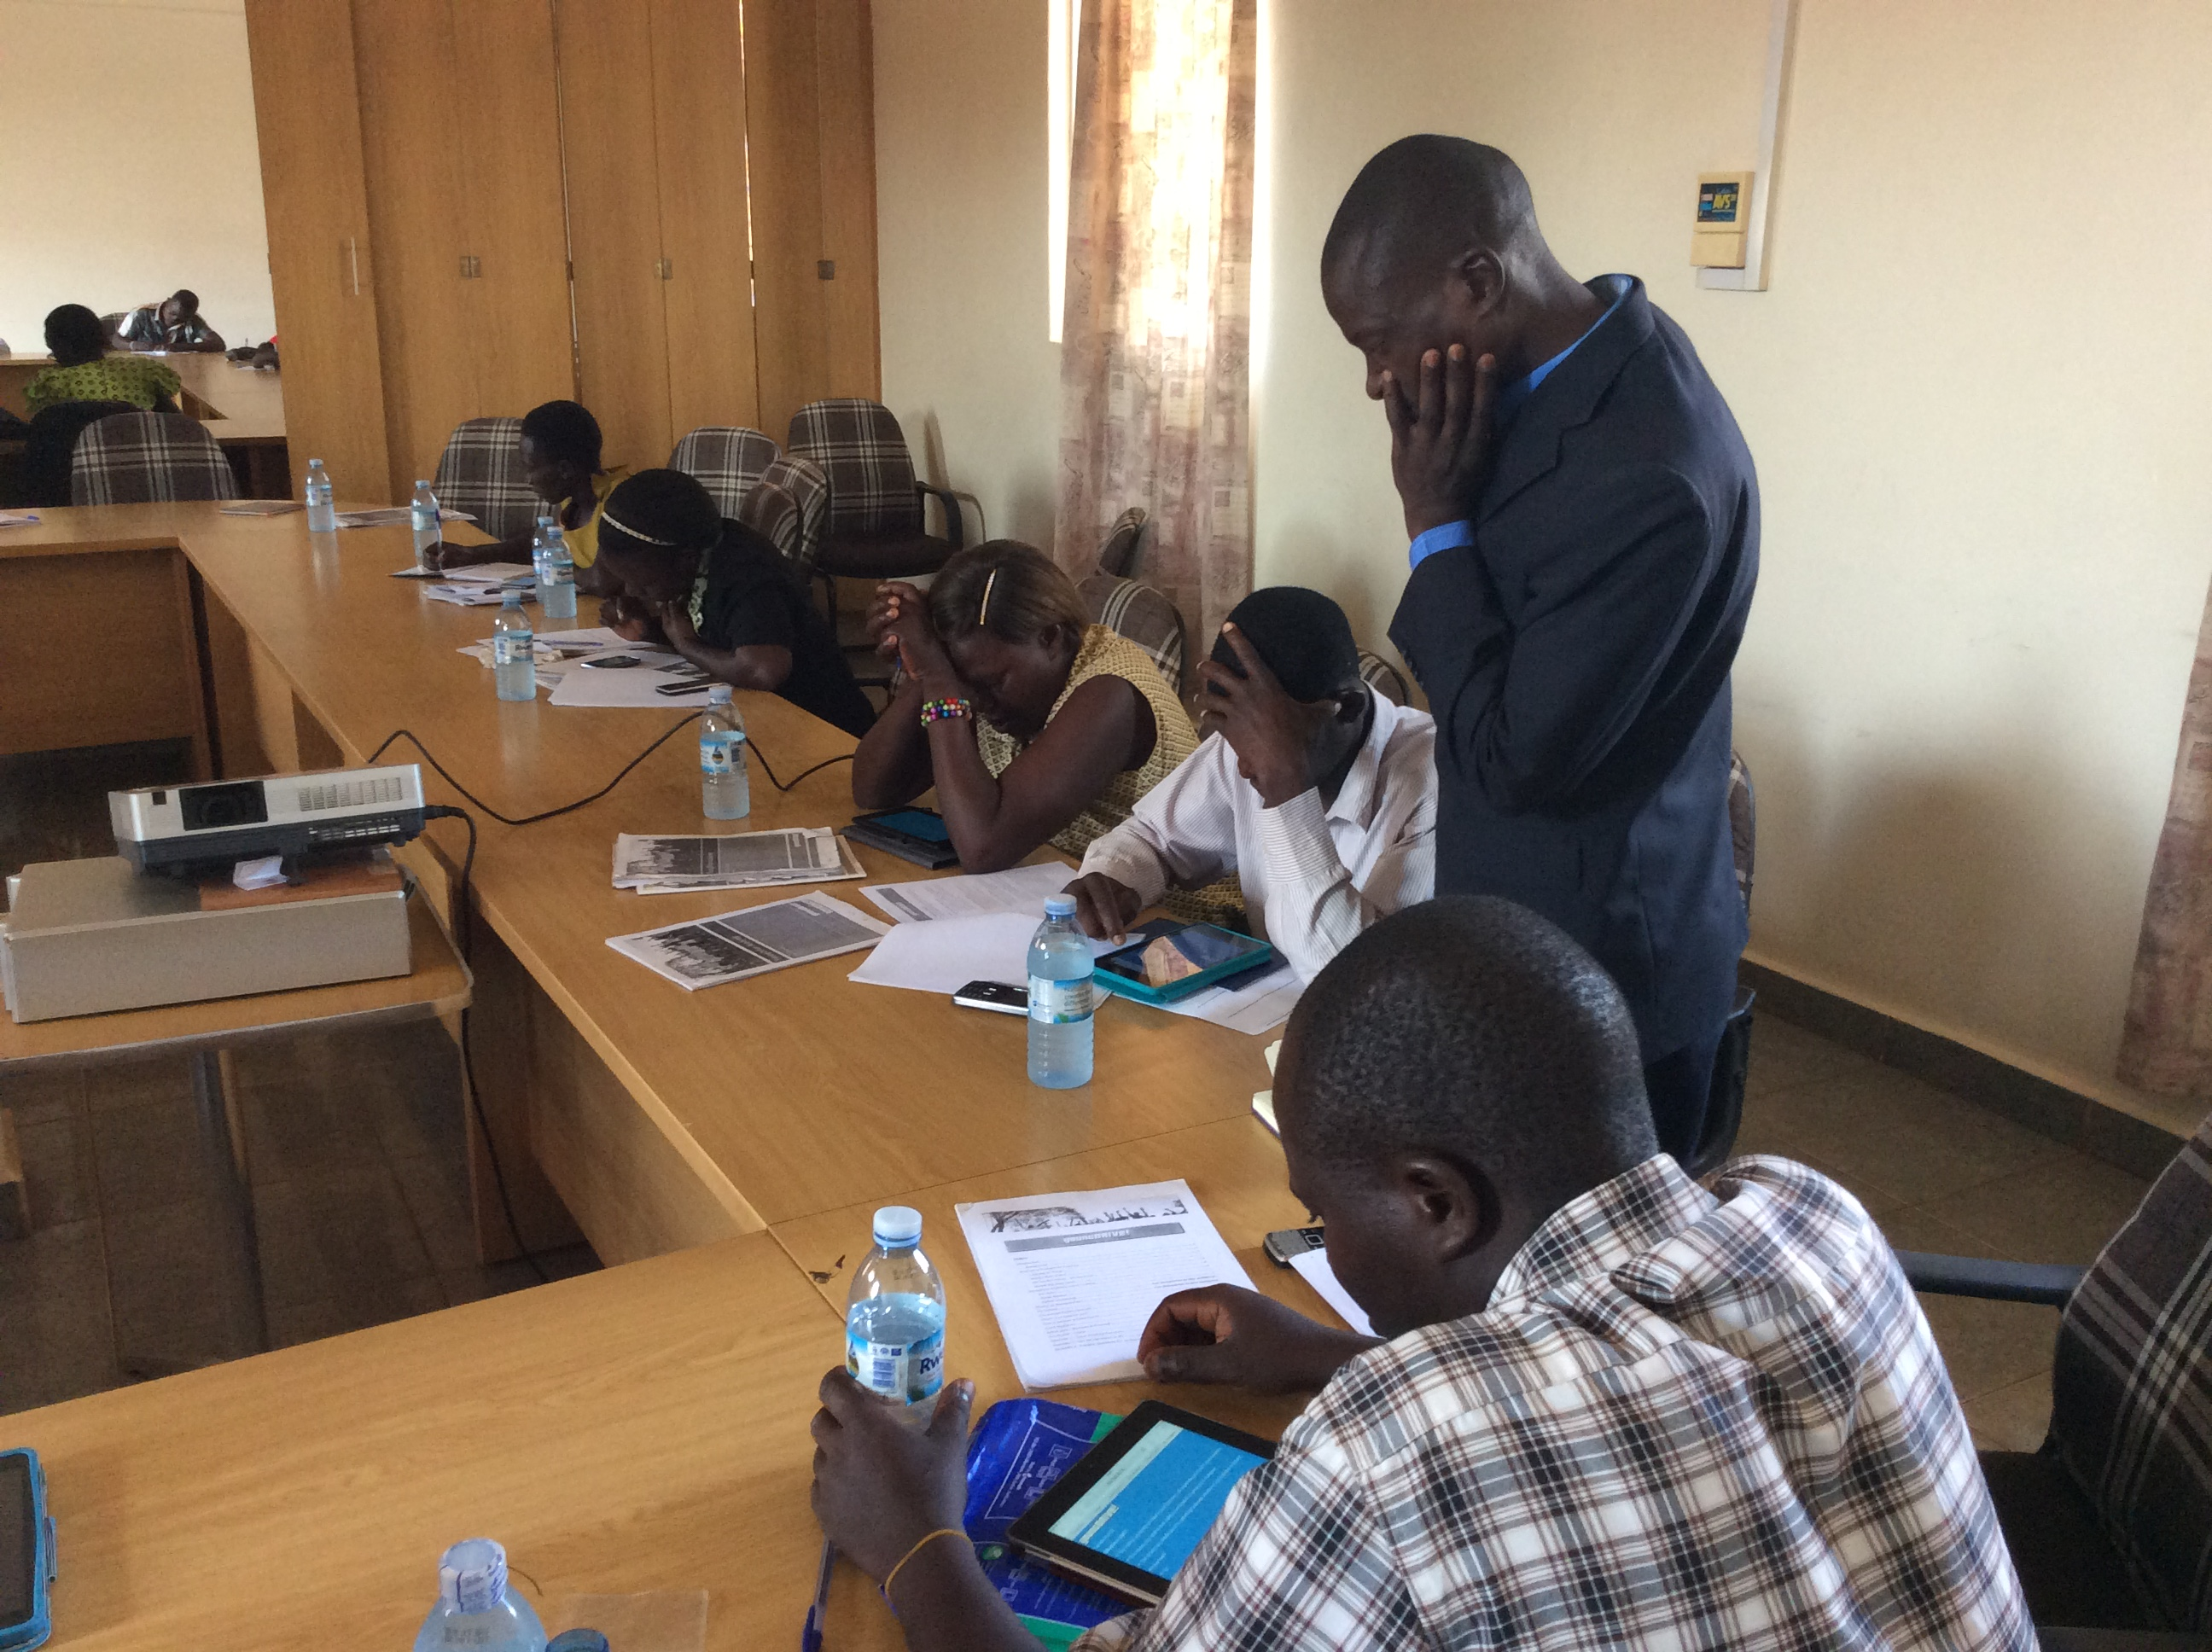
\includegraphics[width=0.7\textwidth]{appevaluation.jpg}
    \caption{Coaches answering the app questions for topic quiz 3 on Financial Literacy, and the coach guide quiz 9 on Action Plan.}
    \label{fig:appevaluation}
\end{figure}

After the test, every coach was divided into one or three groups, on random. In these groups, they were asked:

\begin{enumerate}
\item Why do you think you were correct or incorrect?
\item Do they like the app?
\item Are you stimulated by the app?
\item What did you like?
\item What did you not like?
\item When do you want to use the app?
\item When are you not able to use the app?
\end{enumerate}

To analyse the paper-submitted data, all of this was combined first into a Google Spreadsheet (the app results were also recorded in paper, but only as a backup). Data collection was done by the app itself, which pushes data to server whenever online (it saves quiz start, and quiz finish).

%The next day, a small app evaluation and co-creation workshop was held for the Educator Dashboard, and the final version of the app. Also, a test was done with the Plan Tororo staff.

%Back in Kampala, a presentation was held with Plan International. Back in Sweden, a presentation was held with the YoungDrive Strategic Management Team.

